\documentclass[border=10pt]{standalone}
\usepackage[svgnames]{xcolor}
\usepackage{amsmath}
\usepackage{pgfplots}
\pgfplotsset{compat=newest}
\usepackage[sfdefault]{FiraSans}
\usepackage{FiraMono}
\renewcommand*\familydefault{\sfdefault}
\begin{document}
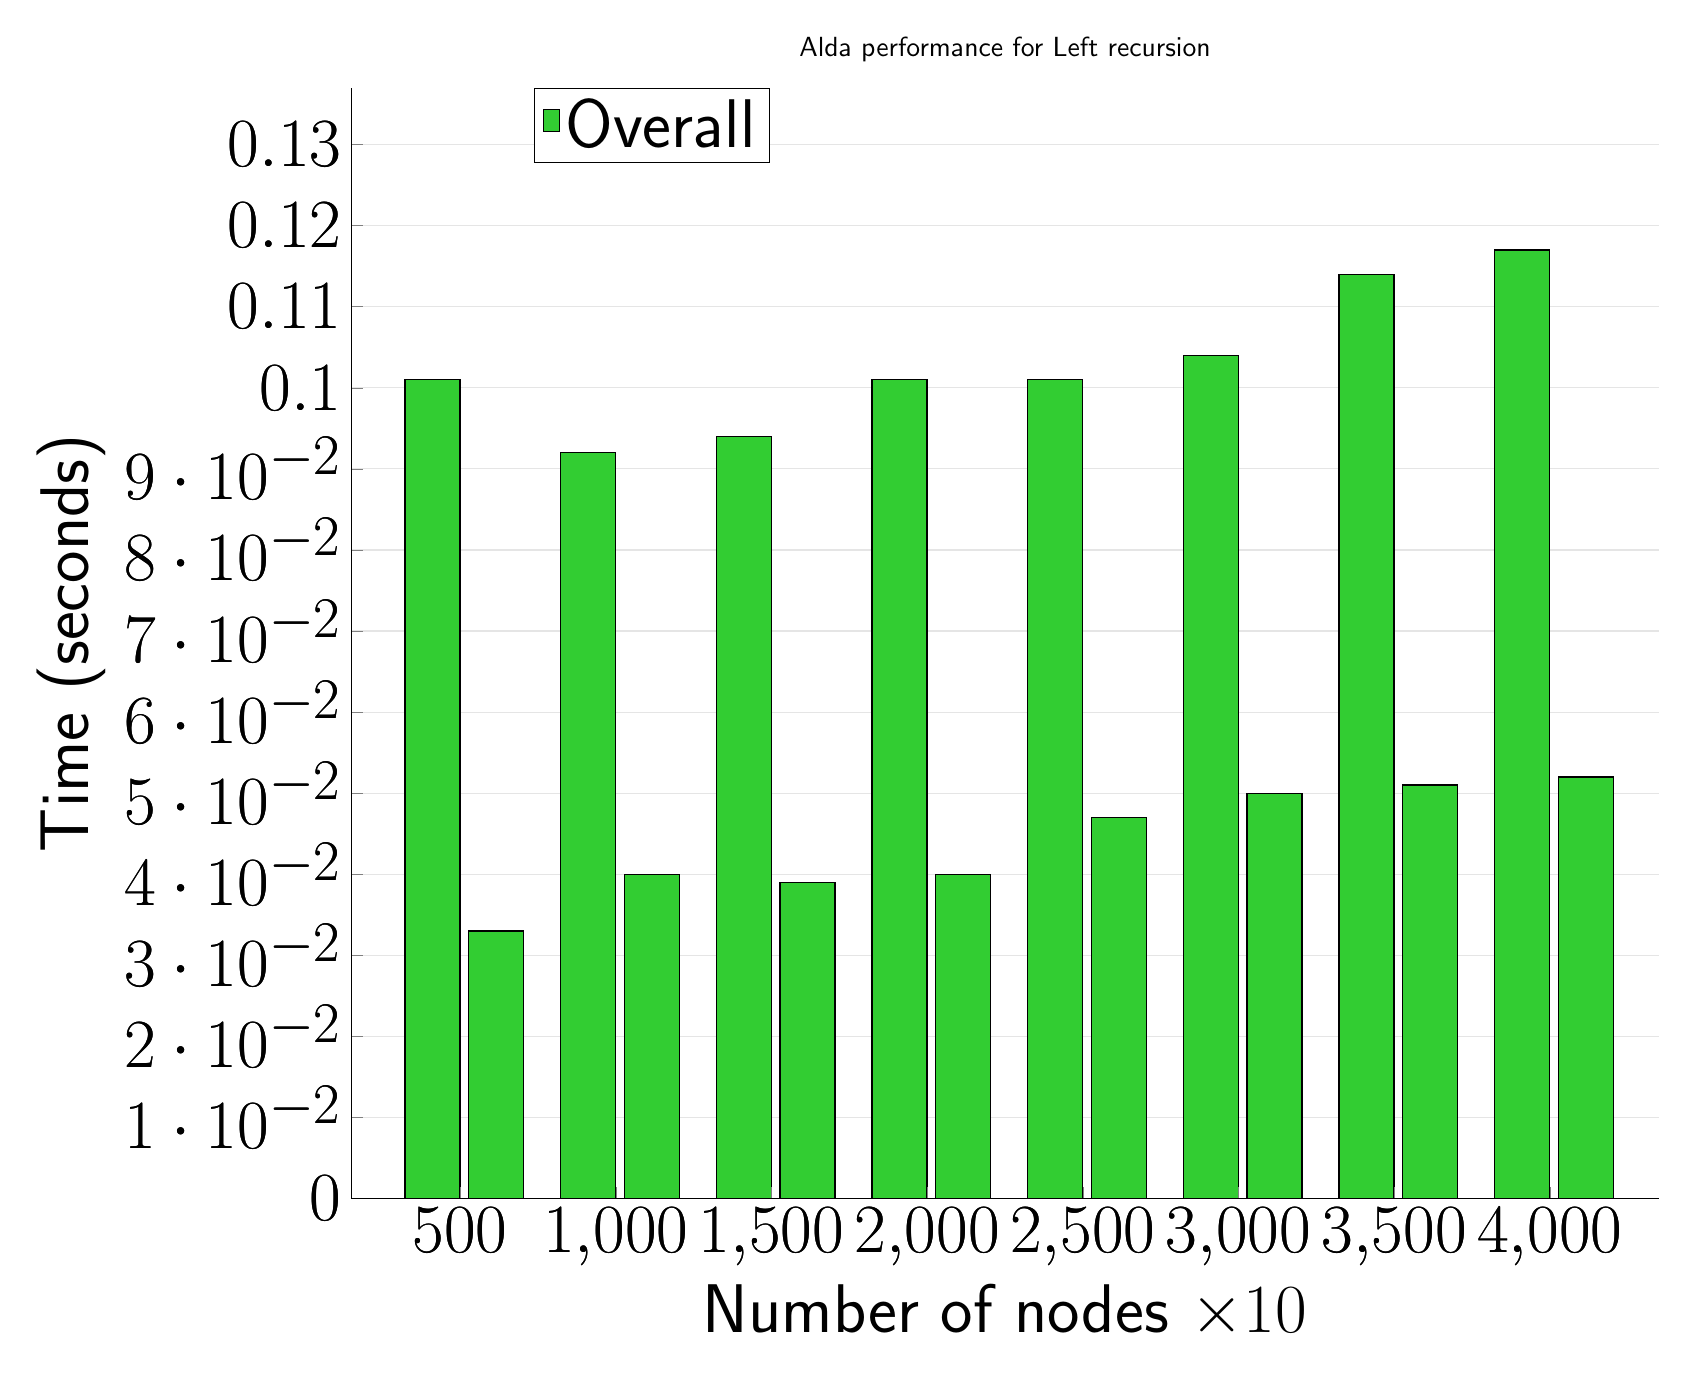
\begin{tikzpicture}
	\begin{axis}[
			ybar stacked,
			title={Alda performance for Left recursion},
			bar shift=-10pt,
			width=1.5\textwidth,
			bar width=0.7cm,
			ymajorgrids, tick align=inside,
			major grid style={draw=gray!20},
			xtick=data,
			ymin=0, ymax=0.13700007915496826,
			axis x line*=bottom,
			axis y line*=left,
			enlarge x limits=0.1,
			legend style={
					at={(0.23, 1)},
					anchor=north,
					legend columns=1,
					font=\Huge,
				},
			ylabel={Time (seconds)},
			xlabel={Number of nodes $\times 10$},
			label style={font=\Huge},
			tick label style={font=\Huge},
		]
		\addlegendimage{fill=LimeGreen, draw=black, line width=0.2pt}
		\addlegendentry{Overall}
		\addplot +[fill=LimeGreen, draw=black, line width=0.5pt] coordinates {
				(500, 0.10099997520446777)
				(1000, 0.09199998378753663)
				(1500, 0.09399998188018799)
				(2000, 0.10100002288818359)
				(2500, 0.10099997520446777)
				(3000, 0.10400006771087647)
				(3500, 0.11399989128112793)
				(4000, 0.11700003147125244)
			};
	\end{axis}
	\begin{axis}[
			ybar stacked,
			bar shift=13pt,
			width=1.5\textwidth,
			bar width=0.7cm,
			ymajorgrids, tick align=inside,
			major grid style={draw=none},
			xtick=data,
			ymin=0, ymax=0.13700007915496826,
			axis x line*=none,
			axis y line*=none,
			enlarge x limits=0.1,
			label style={font=\Huge},
			tick label style={font=\Huge},
		]
		\addplot +[fill=LimeGreen, draw=black, line width=0.5pt] coordinates {
				(500, 0.03300000000000001)
				(1000, 0.040000000000000015)
				(1500, 0.039000000000000014)
				(2000, 0.040000000000000015)
				(2500, 0.047)
				(3000, 0.049999999999999996)
				(3500, 0.051000000000000004)
				(4000, 0.052000000000000005)
			};
	\end{axis}
\end{tikzpicture}

\end{document}
